
% This LaTeX was auto-generated from an M-file by MATLAB.
% To make changes, update the M-file and republish this document.

%%% \documentclass{article}
%%% \usepackage{graphicx}
%%% \usepackage{color}

%%% \sloppy
%%% \definecolor{lightgray}{gray}{0.5}
\setlength{\parindent}{0pt}

%%% \begin{document}

    
    
\subsection*{Signal Spectrum by means of Fast fourier transform}

\begin{par}
Example for algorithm SP-FFT.
\end{par} \vspace{1em}
\begin{par}
Calculates frequency and phase spectrum by means of Fast Fourier Transform algorithm. Result is normalized.
\end{par} \vspace{1em}

\subsubsection*{Contents}

\begin{itemize}
\setlength{\itemsep}{-1ex}
   \item Generate sample data
   \item Call algorithm
   \item Display results
\end{itemize}


\subsubsection*{Generate sample data}

\begin{par}
Two quantities are prepared: \lstinline{y} and \lstinline{fs}, representing 1 second of signal containing 5 harmonic components and one inter-harmonic component. Main signal component has nominal frequency 1 kHz, nominal amplitude 2 V, nominal phase 1 rad and offset 1 V sampled at sampling frequency 10 kHz.
\end{par} \vspace{1em}
\begin{lstlisting}[style=mcode]
DI = [];
fsnom = 1e4; Anom = 2; fnom = 100; phnom = 1; Onom = 0.2;
t = [0:1/fsnom:1-1/fsnom];
DI.y.v = Anom*sin(2*pi*fnom*t + phnom);
for i = 2:45
        DI.y.v = DI.y.v + Anom./i*sin(2*pi*fnom*i*t + phnom + i - 1);
end
DI.y.v = DI.y.v + 1*sin(2*pi*fnom*1.456*t + phnom);
DI.fs.v = fsnom;
\end{lstlisting}


\subsubsection*{Call algorithm}

\begin{par}
Use QWTB to apply algorithm \lstinline{SP-FFT} to data \lstinline{DI}.
\end{par} \vspace{1em}
\begin{lstlisting}[style=mcode]
DO = qwtb('SP-FFT', DI);
\end{lstlisting}

        \begin{lstlisting}[style=output]
QWTB: no uncertainty calculation
\end{lstlisting} \color{black}
    

\subsubsection*{Display results}

\begin{par}
Results is the amplitude and phase spectrum.
\end{par} \vspace{1em}
\begin{lstlisting}[style=mcode]
figure
plot(DO.f.v, DO.A.v, '-x')
xlabel('f (Hz)'); ylabel('A (V)'); title('Amplitude spectrum of the signal');
figure
plot(DO.f.v, DO.ph.v, '-x')
xlabel('f (Hz)'); ylabel('phase (rad)'); title('Phase spectrum of the signal');
\end{lstlisting}

\begin{center}
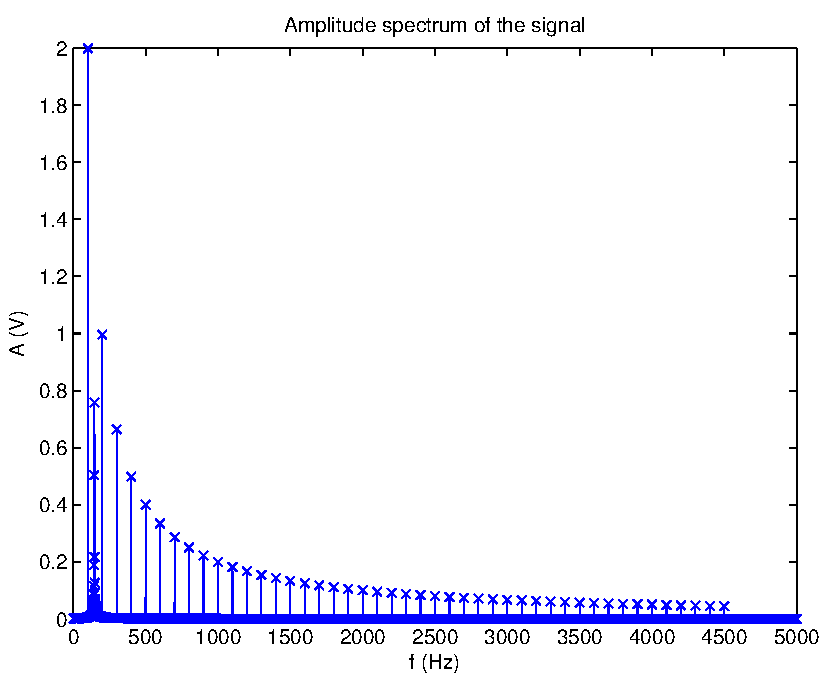
\includegraphics[width=0.7\textwidth]{alg_examples_published/SP-FFT_alg_example_01.pdf}
\end{center}

\begin{center}
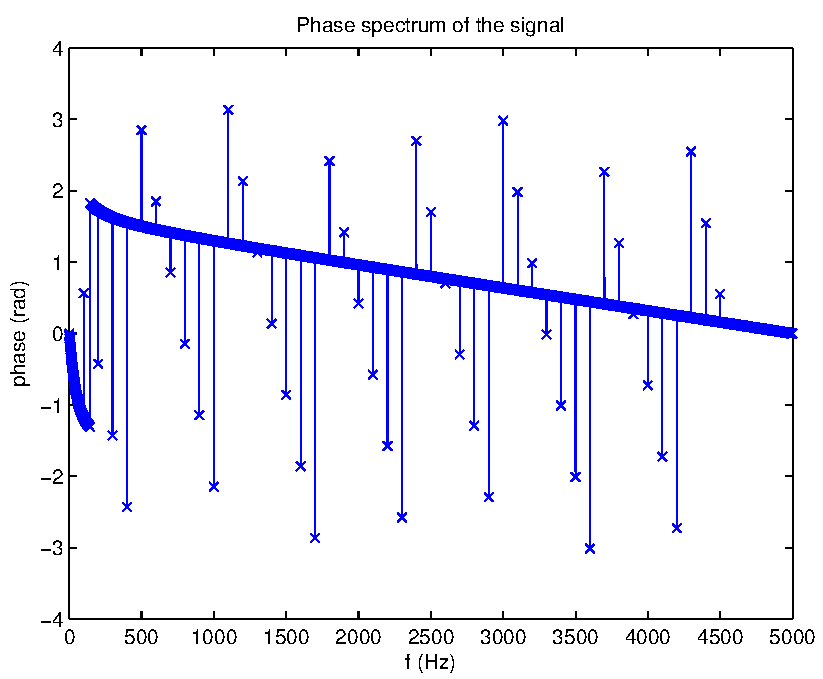
\includegraphics[width=0.7\textwidth]{alg_examples_published/SP-FFT_alg_example_02.pdf}
\end{center}



%%% \end{document}
    
